\section{РАЗРАБОТКА БАЗЫ ДАННЫХ}
\subsection{Концептуальная модель}

Предметная область - совокупность объектов,
свойства которых и отношения между которыми рассматриваются в рамках некоторого исследования.

Модель предметной области – некоторая система, адекватно имитирующая
структуру и функционирование исследуемой предметной области.

Концептуальная модель - это структура моделируемой предметной области,
свойств её элементов и причинно-следственных связей, присущих системе и
существенных для достижения цели моделирования.
В рамках этапа концептуального моделирования выделяются основные смысловые единицы (сущности)
предметной области, определяются и описываются связи между ними.

Концептуальная модель ориентирована на потенциальных пользователей базы данных,
так как представляет предметную область на их уровне понимания.
Этот уровень называется системно-независимым или предметно-ориентированным.

\subsubsection{ЛКМ для БП <<Приказ о создании комиссии инвентаризационной>>}

Локальная концептуальная модель для бизнес процесса с документом <<Приказ о создании комиссии инвентаризационной>>
изображена на рисунке~\ref{fig:LKM_PrikazSozdKomInvent}.

\begin{figure}[!h]
    \centering
    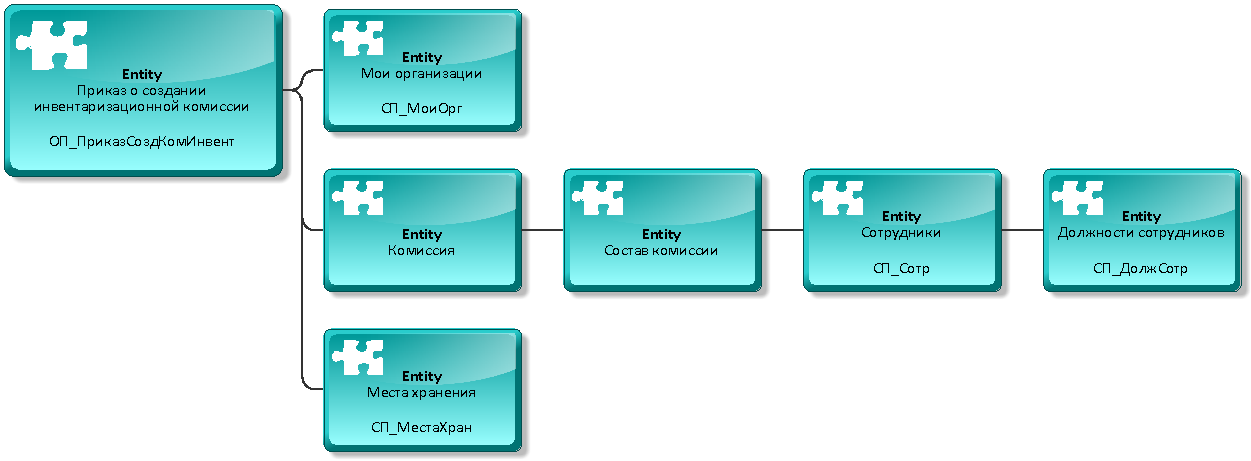
\includegraphics[width=18cm]
        {_docs/ЛКМ_ПриказСоздКомИнвент.png}
    \caption{Локальная концептуальная модель для бизнес процесса с документом <<Приказ о создании комиссии инвентаризационной>>}
    \label{fig:LKM_PrikazSozdKomInvent}
\end{figure}

\newpage

\subsubsection{ЛКМ для БП <<Инвентаризационная опись>>}

Локальная концептуальная модель для бизнес процесса с документом <<Инвентаризационная опись>>
изображена на рисунке~\ref{fig:LKM_InvenOpis}.

\begin{figure}[!h]
    \centering
    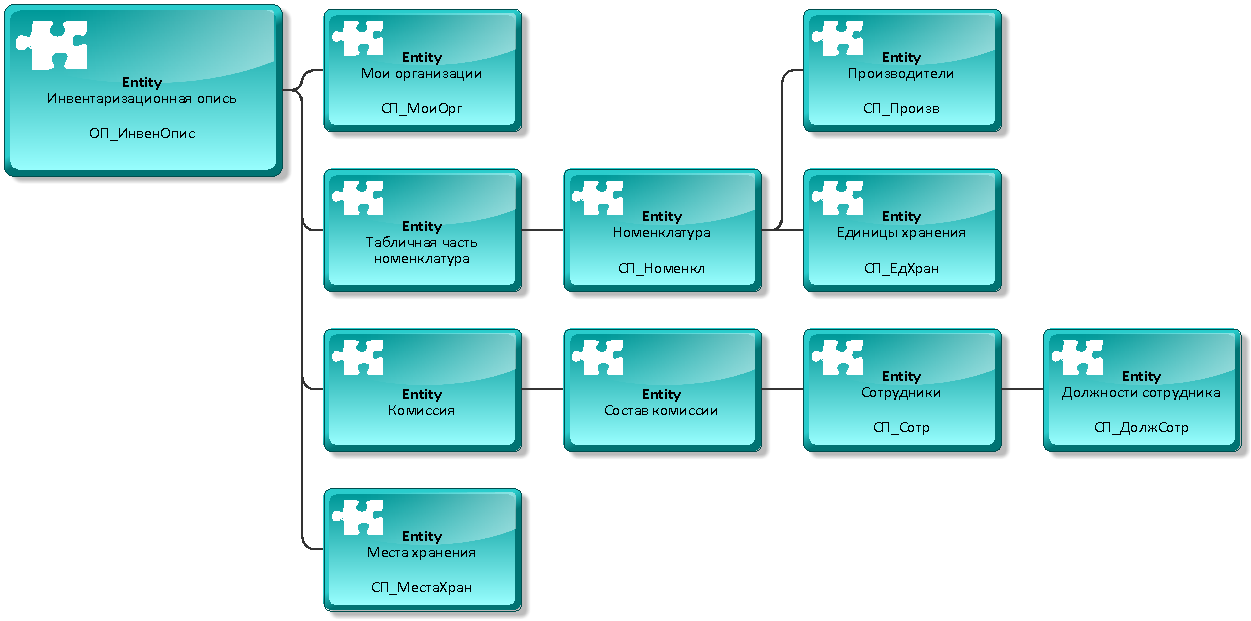
\includegraphics[width=18cm]
        {_docs/ЛКМ_ИнвенОпис.png}
    \caption{Локальная концептуальная модель для бизнес процесса с документом <<Инвентаризационная опись>>}
    \label{fig:LKM_InvenOpis}
\end{figure}

\newpage
\subsubsection{КМ для БП ОА}

Концептуальная модель для бизнес-процесса объекта автоматизации <<Инвентаризация>>
изображена на рисунке~\ref{fig:KM}.

\begin{figure}[!h]
    \centering
    \includegraphics[width=18cm]
        {_docs/КМ.png}
    \caption{Концептуальная модель}
    \label{fig:KM}
\end{figure}

\newpage
\subsection{Логическая модель}

Логическая модель 
изображена на рисунке~\ref{fig:KM}.

\begin{figure}[!h]
    \centering
    \includegraphics[width=18cm]
        {_docs/ЛМ.png}
    \caption{Логическая модель}
    \label{fig:LM}
\end{figure}

\newpage
\subsection{Физическая модель}

\lstinputlisting[language=sql]
    {src/create_database.sql}

\lstinputlisting[language=sql]
    {src/delete_database.sql}

\newpage
